Fast graph loading is important for efficient graph processing due to the high ratio of irregular memory accesses to actual computation in graph applications. This performance limitation is largely due to the memory bandwidth of today's machines. As modern IO is fast compared to CPU performance, and storage capacities and bandwidth are increasing, CPUs are not as fast as they used to be. Therefore, loading graphs quickly becomes crucial for efficient processing. For instance, the paper "A Distributed Multi-GPU System for Fast Graph Processing" presents Lux, a system that achieves fast graph processing by exploiting the aggregate memory bandwidth on GPUs, achieving up to 20 times speedup over shared memory systems. Similarly, "Efficient Large-Scale Graph Processing on Hybrid CPU and GPU Systems" demonstrates that partitioning large-scale graphs to be processed concurrently on hybrid CPU and GPU platforms offers significant performance gains. Additionally, "GRAPE for fast and scalable graph processing and random-walk-based embedding" shows that GRAPE is faster and requires less memory than state-of-the-art libraries for loading large graphs. Therefore, fast graph loading is crucial for efficient graph processing, especially as graph sizes and complexities continue to grow.

% -Reduced power-bill, and reduced cloud charges

% Reintro
Graphs are fundamental data structures in many applications, such as social networks, recommendation systems, and biological networks. Fast graph loading is crucial for minimizing the time it takes to start processing and analyzing the graph data. Loading graph data can be a significant bottleneck in graph processing workflows. Efficient loading becomes crucial as the cost of loading data can dominate the overall processing time, especially as computational capabilities continue to improve. Some existing graph processing frameworks may face challenges in terms of efficiency during the loading phase. Optimization of these frameworks is essential to harness the full potential of modern hardware. As you mentioned, modern IO technologies, increased storage capacities, and high bandwidths have enabled faster data loading. Utilizing these advancements is essential for improving overall graph processing performance. The increasing gap between CPU performance and storage capabilities underscores the importance of optimizing data loading processes. Efficient utilization of high-speed storage can compensate for the relatively slower improvements in CPU speeds.

The choice of graph file format affects loading speed. COO (Coordinate List), MTX (Matrix Market), and other formats have different characteristics, and selecting an appropriate format based on the application and storage considerations is crucial. Memory storage formats, such as Edgelist and CSR (Compressed Sparse Row), impact the efficiency of graph processing algorithms. Choosing the right format can lead to significant performance improvements during both loading and computation.


% EMAIL
Gunrock is the slowest here, followed by cuhornet, the one i am working on, and PIGO. PIGO is still ~8x faster than my implementation, but it does not support dynamic updates while my implementation does. Reducing loading time in important to enable faster iterations upon our algorithms.
My implementation inserts into a 2d-vector (or a vector of vectors) and ensures sorted and unique keys upon call to update(). This is faster than doing a binary search upon each addEdge() to check for an edge's existence. I use a custom unique\_merge() function for this - using a small buffer (a bufferless merge is inefficient).

I tried a simple file bytes sum using mmap() - both sequential and parallel using openmp (64 threads on DGX). I adjust madvise(), mmap(), and per-thread block size to see which access pattern has the best performance.
It seems to me using an early madvice(MADV\_WILLNEED), a per-thread block size of 256K (dynamic schedule) is good. Below is a plot showing the time taken with this config for each graph.

In parallel doing a file byte sum takes ~100ms on indochina-2004 graph. Note that PIGO takes ~650ms to load the same graphs as CSR. Next i measure the read bandwith of each file, simply by dividing the size of each file by the time taken.

We appear to be reaching a peak bandwidth of ~35GB/s. The KIOXIA KCM6DRUL7T68 7.68TB NVMe SSD installed on DGX has a peack sequential read performance of 62GB/s (we are close). Sequential approach can hit a max of only 6GB/s.
https://www.acmemicro.com/Product/17847/Kioxia-KCD6XLUL7T68---7-68TB-SSD-NVMe-2-5-inch-15mm-CD6-R-Series-SIE-PCIe-4-0-6200-MB-sec-Read-BiCS-FLASH-TLC-1-DWPD

There is a paper called "Efficient Memory Mapped File I/O for In-Memory File Systems" on the topic - where Choi et al. working at Samsung say that mmap() is a good interface for fast IO (in contrast to file streams) and propose async map-ahead based madvise() for low-latency NVM storage devices. The also have a good slides on this - where their (modified) extended madvice obtains ~2.5x better performance than default mmap() by minimizing the number of page faults.

I tried parsing integers from text and saving into per-thread integer lists. To over-allocate memory for per-thread integer-lists i use sufficient size mmap() instead of malloc(). Even if i over-allocate, due to virtual memory, only memory as much i need is actually used.


% - Why fast graph loading is important?
% - Extremely high cost of loading compared to computation.
% - An issue with even popular graph processing frameworks.
% - Modern IO is fast (compared to CPU performance).
% - Storage capacities increasing, bandwidth is high, CPUs as not as fast as they used to be.
% - Common graph file formats (COO, MTX).
% - Common memory storage formats (Edgelist, CSR).
% - Work presented in this paper.




%% - Use --- for a dash.
%% - Use ``camera-ready'' for quotes.
%% - Use {\itshape very} or \textit{very} for italicized text.
%% - Use \verb|acmart| or {\verb|acmart|} for mono-spaced text.
%% - Use \url{https://capitalizemytitle.com/} for URLs.
%% - Use {\bfseries Do not modify this document.} for important boldface details.
%% - Use \ref{fig:name} for referencing.

%% For a block of pre-formatted text: 
% \begin{verbatim}
%   \renewcommand{\shortauthors}{McCartney, et al.}
% \end{verbatim}

%% For a list of items:
% \begin{itemize}
% \item the ``ACM Reference Format'' text on the first page.
% \item the ``rights management'' text on the first page.
% \item the conference information in the page header(s).
% \end{itemize}

%% For a table:
% \begin{table}
%   \caption{Frequency of Special Characters}
%   \label{tab:freq}
%   \begin{tabular}{ccl}
%     \toprule
%     Non-English or Math&Frequency&Comments\\
%     \midrule
%     \O & 1 in 1,000& For Swedish names\\
%     $\pi$ & 1 in 5& Common in math\\
%     \$ & 4 in 5 & Used in business\\
%     $\Psi^2_1$ & 1 in 40,000& Unexplained usage\\
%   \bottomrule
% \end{tabular}
% \end{table}

%% For a full-width table:
% \begin{table*}
%   \caption{Some Typical Commands}
%   \label{tab:commands}
%   \begin{tabular}{ccl}
%     \toprule
%     Command &A Number & Comments\\
%     \midrule
%     \texttt{{\char'134}author} & 100& Author \\
%     \texttt{{\char'134}table}& 300 & For tables\\
%     \texttt{{\char'134}table*}& 400& For wider tables\\
%     \bottomrule
%   \end{tabular}
% \end{table*}


%% For inline math:
% \begin{math}
%   \lim_{n\rightarrow \infty}x=0
% \end{math},

%% For a numbered equation:
% \begin{equation}
%   \lim_{n\rightarrow \infty}x=0
% \end{equation}

%% For an unnumbered equation:
% \begin{displaymath}
%   \sum_{i=0}^{\infty} x + 1
% \end{displaymath}

%% For a figure:
% \begin{figure}[h]
%   \centering
%   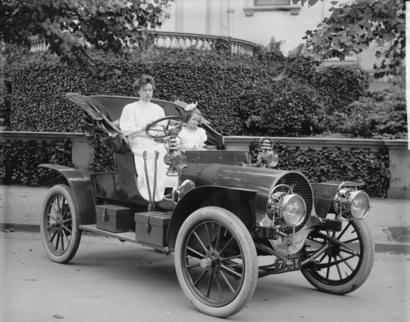
\includegraphics[width=\linewidth]{inc/sample-franklin}
%   \caption{1907 Franklin Model D roadster. Photograph by Harris \&
%     Ewing, Inc. [Public domain], via Wikimedia
%     Commons. (\url{https://goo.gl/VLCRBB}).}
%   \Description{A woman and a girl in white dresses sit in an open car.}
% \end{figure}

%% For a teaser figure.
% \begin{teaserfigure}
%   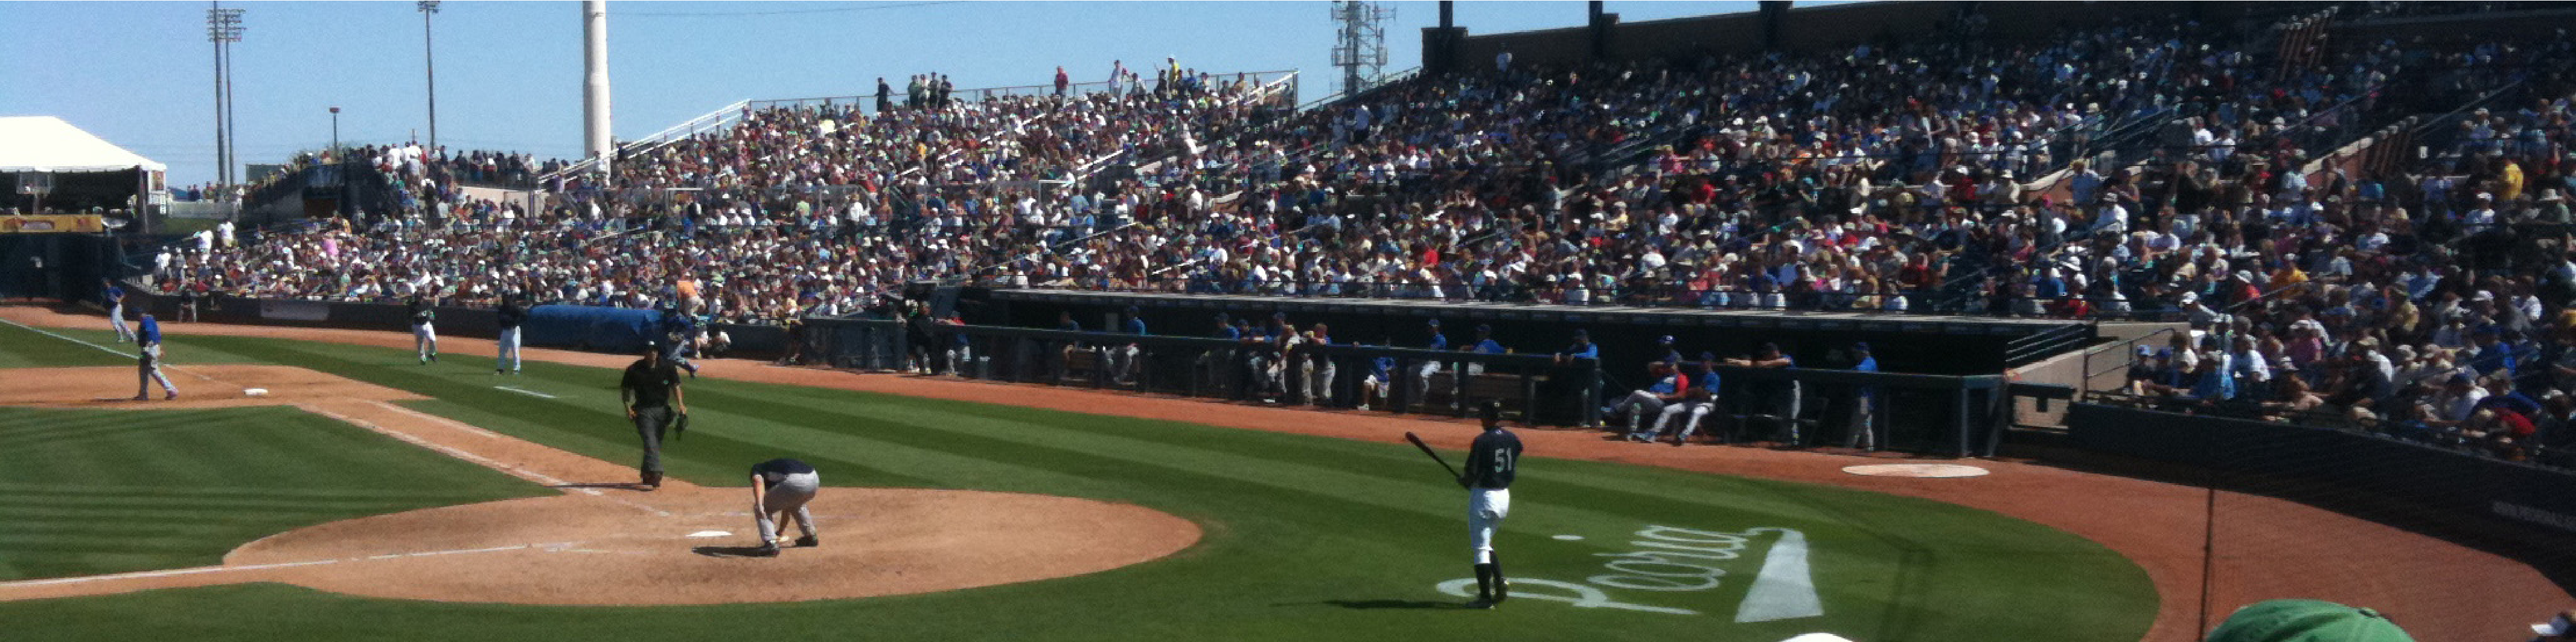
\includegraphics[width=\textwidth]{sampleteaser}
%   \caption{figure caption}
%   \Description{figure description}
% \end{teaserfigure}
